\mySection{9.2 Testing $H_0:\mu_X=\mu_Y$}
%-------------- start slide -------------------------------%{{{ 9.26
\begin{frame}
	% {\S\: 9.2 Testing $H_0:\mu_X=\mu_Y$}
\begin{itemize}
	\item Let $X_1,\cdots, X_n$ be a random sample of size $n$ from $N(\mu_X,\sigma^2_X)$.	\\[1em]
	\item Let $Y_1,\cdots, Y_m$ be a random sample of size $m$ from $N(\mu_Y,\sigma^2_Y)$.
\end{itemize}
\vfill
\begin{center}
\begin{minipage}{0.5\textwidth}
\begin{enumerate}
	\item[Prob. 1] Testing $H_0:\mu_X=\mu_Y$ if $\sigma_X^2 = \sigma_Y^2$. \\[3em]
	\item[Prob. 2] Testing $H_0:\mu_X=\mu_Y$ if $\sigma_X^2 \ne \sigma_Y^2$.
\end{enumerate}
\end{minipage}
\end{center}
\vfill
\mySeparateLine
\vfill

\begin{minipage}{0.4\textwidth}
	\begin{itemize}
		\item True means: \hfill $\mu_X$, $\mu_Y$
		\item True std. dev.'s: \hfill $\sigma_X$, $\sigma_Y$
		\item True variances:\hfill  $\sigma_X^2$, $\sigma_Y^2$\\[2em]
		% \item Sample means:\hfill  $\overline{X}$, $\overline{Y}$
		% \item Sample std. dev.'s: \hfill $S_X$, $S_Y$
		% \item Sample variances: \hfill $S_X^2$, $S_Y^2$
	\end{itemize}
\end{minipage}
\hfill
\begin{minipage}{0.45\textwidth}
	\begin{itemize}
		% \item True means: \hfill $\mu_X$, $\mu_Y$
		% \item True std. dev.'s: \hfill $\sigma_X$, $\sigma_Y$
		% \item True variances:\hfill  $\sigma_X^2$, $\sigma_Y^2$\\[2em]
		\item Sample means:\hfill  $\overline{X}$, $\overline{Y}$
		\item Sample std. dev.'s: \hfill $S_X$, $S_Y$
		\item Sample variances: \hfill $S_X^2$, $S_Y^2$
	\end{itemize}
\end{minipage}
\end{frame}
%-------------- end slide -------------------------------%}}}
%-------------- start slide -------------------------------%{{{ 9.27
\begin{frame}{When $\sigma_X^2=\sigma_Y^2 = \sigma^2$}
\begin{itemize}
	\item[Def.] The \textcolor{yellow!80!black}{\bf pooled variance}:
		$\displaystyle S_p^2 =\frac{(n-1)S_X^2+(m-1)S_Y^2}{n+m-2}$\\[2em]
	\hspace{11.5em} $\displaystyle
	= \frac{\sum_{i=1}^n (X_i-\overline{X})^2+ \sum_{j=1}^n (Y_j-\overline{Y})^2 }{n+m-2}$
\vfill
\item[Thm.]
$\displaystyle T_{n+m-2}=\frac{\overline{X}-\overline{Y}-(\mu_X-\mu_Y)}{S_p\sqrt{ \frac{1}{n}+\frac{1}{m} }}$
$\sim$
Student t distr. of $n+m-2$ dgs of fd.
\vfill
\item[Proof.] (See slides on Section 9.1) \myEnd
\end{itemize}
\end{frame}
%-------------- end slide -------------------------------%}}}
%-------------- start slide -------------------------------%{{{ 9.28
\begin{frame}{When $\sigma_X^2=\sigma_Y^2 = \sigma^2$}

\centering
Testing $H_0:\mu_X = \mu_Y$ v.s.\\[1em]
(at the $\alpha$ level of significance)
\\[1em]
$\displaystyle t=\frac{\bar{x}-\bar{y}}{s_p\sqrt{ \frac{1}{n}+\frac{1}{m} }}$
\vfill

\begin{minipage}{0.32\textwidth}
\centering
$H_1:\mu_X <\mu_Y$:\\[1em]
Reject $H_0$ if \\[1em]
$t \le -t_{\alpha,n+m-2}$
\end{minipage}
\begin{minipage}{0.32\textwidth}
\centering
$H_1:\mu_X \ne \mu_Y$:\\[1em]
Reject $H_0$ if \\[1em]
$|t| \ge t_{\alpha/2,n+m-2}$
\end{minipage}
\begin{minipage}{0.32\textwidth}
\centering
$H_1:\mu_X>\mu_Y$:\\[1em]
Reject $H_0$ if \\[1em]
$t \ge t_{\alpha,n+m-2}$
\end{minipage}
\end{frame}
%-------------- end slide -------------------------------%}}}
%-------------- start slide -------------------------------%{{{ 9.29
\begin{frame}
\begin{itemize}
\item[E.g.] Test whether Mark Twain and Snodgrass are the same person by checking the proportion of three-letter words at the $99\%$ level of significance.
\begin{center}
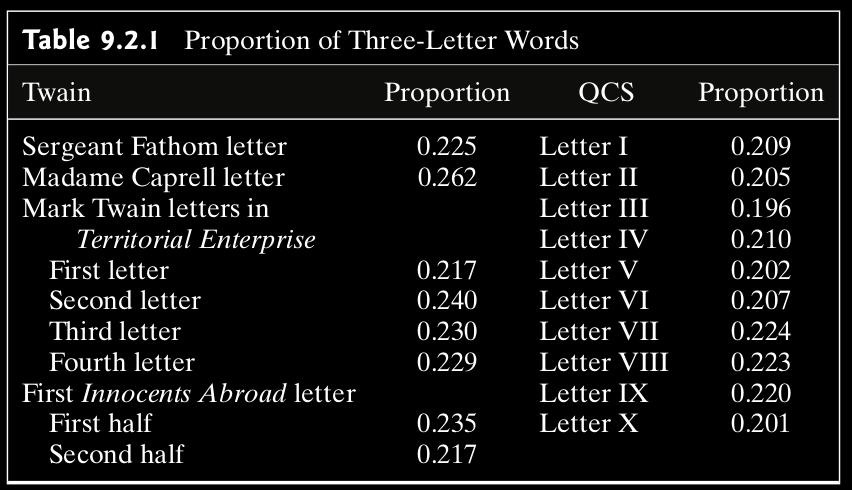
\includegraphics[scale=0.2]{Table_9-2-1-neg.png}
\end{center}
\vfill
\item[Sol.] We need to test
	\[
	H_0: \mu_X = \mu_Y \quad v.s. \quad H_1: \mu_X\ne \mu_Y.
	\]
	Since we are tesing whether they are the same person, one can assume that $\sigma_X^2 = \sigma_Y^2$.
\end{itemize}
\end{frame}
%-------------- end slide -------------------------------%}}}
%-------------- start slide -------------------------------%{{{ 9.30
\begin{frame}
\begin{enumerate}
\item $n=8$, $m=10$,
\begin{align*}
&\sum_{i=1}^n x_i = 1.855,\quad \sum_{i=1}^n x_i^2 = 0.4316\\
&\sum_{i=1}^m y_i = 2.097,\quad \sum_{i=1}^m y_i^2 = 0.4406
\end{align*}
\vfill
\item Hence,
	\[
		\bar{x} = 1.855/8=02319 \quad \bar{y}=2.097/10 =0.2097
	\]
	\[
		s_X^2 =  \frac{8\times 0.4316-1.855^2}{8\times 7}=0.0002103
	\]
	\[
		s_Y^2 =  \frac{10\times 0.4406-2.097^2}{10\times 9}=0.0000955
	\]
	\[
		s_p^2 =  \frac{(n-1)s_X^2+(m-1)s_Y^2}{n+m-2} =...=0.0001457
	\]
	\[
		t=  \frac{\bar{x}-\bar{y}}{s_p\sqrt{ \frac{1}{n}+ \frac{1}{m} }} = ... = 3.88
	\]
\end{enumerate}
\end{frame}
%-------------- end slide -------------------------------%}}}
%-------------- start slide -------------------------------%{{{ 9.31
\begin{frame}
	\begin{itemize}
		\item[3.] Critical region: $|t|\ge t_{0.005,n+m-2} = t_{0.005,16} = 2.9208$. \\[1em]
			\begin{center}
				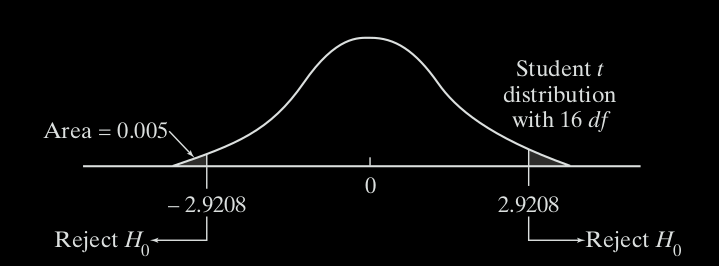
\includegraphics[scale=0.3]{Figure_9-2-1-neg.png}
			\end{center}
		 \vfill
		\item[4.] Conclusion: Rejection! \myEnd
	\end{itemize}
\end{frame}
%-------------- end slide -------------------------------%}}}
%-------------- start slide -------------------------------%{{{ 9.32
\begin{frame}

	\begin{enumerate}
		\item[E.g.] Comparing large-scales and small-scales companies:\\[1em]
			Based on the data below, can we say that the return o equity differs between the two types of companies?
			\vfill
			\begin{center}
			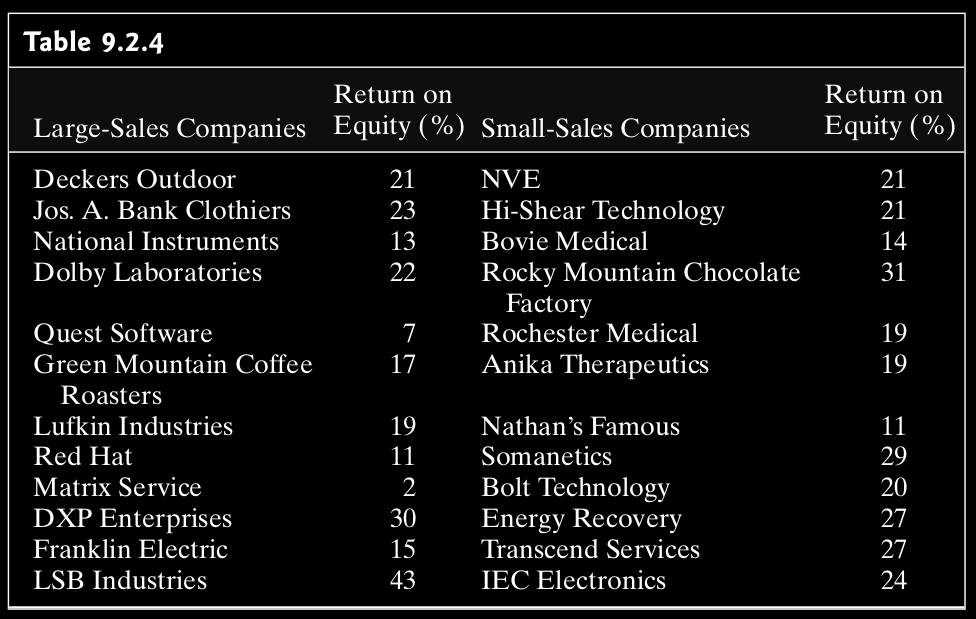
\includegraphics[scale=0.2]{Table_9-2-4-neg.png}
			\end{center}
	\end{enumerate}
\end{frame}
%-------------- end slide -------------------------------%}}}
%-------------- start slide -------------------------------%{{{ 9.33
\begin{frame}
	\begin{enumerate}
		\item[Sol.] Let $\mu_X$ and $\mu_Y$ be the average returns. We are asked to test\\[1em]
			\[
			H_0: \mu_X = \mu_Y \qquad v.s. \qquad H_1: \mu_X\ne \mu_Y.
			\]
			\vfill
		\item[1.]
			\[
			n=12,\qquad	\sum_{i=1}^n x_i = 223
				\qquad
				\sum_{i=1}^n x_i^2 = 5421
			\]
			\[
			m=12,\qquad	\sum_{i=1}^m y_i = 263
				\qquad
				\sum_{i=1}^m y_i^2 = 6157
			\]
		\item[2.]
			\[
				\bar{x} = 18.5833,\qquad s_X^2 = 116.0833
			\]
			\[
				\bar{y} = 21.9167, \qquad s_Y^2 = 35.7197
			\]
			\[
				w= \frac{18.5833 -21.9167 }{\sqrt{ \frac{116.0833}{12}+  \frac{35.7197}{12} }} = -0.9371932.
			\]
			\[
				\hat\theta =  \frac{116.0833}{35.7179} = 3.250 \quad\Rightarrow\quad
				\nu = \left[ \frac{(3.250+1)^2}{ \frac{1}{11}3.250^2+ \frac{1}{11} 1^2 } \right]
				=\left[ 17.18403\right] = 17.
			\]
	\end{enumerate}
\end{frame}
%-------------- end slide -------------------------------%}}}
%-------------- start slide -------------------------------%{{{ 9.34
\begin{frame}
	\begin{itemize}
		\item[3.] The critical region is $|w|\ge t_{\alpha/2,17} = 2.1098$.\\[2em]
		\item[4.] Conclusion: \\[1em] Since $w= -0.94$ is not in the critical region, we fail to reject $H_0$. \myEnd
	\end{itemize}
\end{frame}
%-------------- end slide -------------------------------%}}}
